\section{Local template matching}

\begin{frame}
	\frametitle{Local template matching}
	\begin{itemize}
		\item Kernel machines prototypical template matchers
		\begin{displaymath}
			f(x) = b + \sum_{i} \alpha_i K(\mathbf{x},\mathbf{x}_i)
		\end{displaymath}
		kernel $K(\cdot,\mathbf{x}_i)$ gives similarity
		\item Local kernel $K$ generalizes by using \emph{smoothness prior}: Target function $f(\mathbf{x})$ is influenced by training values $f(\mathbf{x}_i)$ in neighbourhood
		\item Implicit separation of input space in regions for which a smooth function is estimated
		\item If target function is highly varying, then many examples required to catch all twists and turns
		\note[item]{Highly varying: piecewise linear approximation would require a large number of pieces}
	\end{itemize}
\end{frame}

\begin{frame}
	\frametitle{Highly varying functions in AI-set?}
	\begin{itemize}
		\item Consider recognition of shifted letters
		\item All shifted letters of the same class lie on a non-linear manifold with high curvature
	\end{itemize}
	\begin{figure}
		\centering
		\includegraphics[width=7cm]{images/shiftingW.png}
	\end{figure}
\end{frame}

\begin{frame}
	\frametitle{Varying functions contd.}
	\begin{figure}
		\centering
		\includegraphics[width=7cm]{images/tangentVectors.png}
	\end{figure}
	\begin{itemize}
		\item Difference images (tangent vectors) orthogonal $\Rightarrow$ Indication for high curvature
	\end{itemize}
\end{frame}

\begin{frame}
	\frametitle{Implications}
\end{frame}
